\chapter{Introduction and Background Research}

% You can cite chapters by using '\ref{chapter1}', where the label must
% match that given in the 'label' command, as on the next line.
\label{chapter1}

% Sections and sub-sections can be declared using \section and \subsection.
% There is also a \subsubsection, but consider carefully if you really need
% so many layers of section structure.
\section{Introduction}

%<A brief introduction suitable for a non-specialist, {\em i.e.} without using technical terms or jargon, as far as possible. This may be similar/the same as that in the 'Outline and Plan' document. The remainder of this chapter will normally cover everything to be assessed under the `Background Research` criterion in the mark scheme.>

%{\em** Start by explaining the problem. This includes a brief description of PDEs, the need for numerical solutions to such equations and general motivation for the subject. Then go on to talk about the need for education, future aims for the project (such as being turned into a module or maybe a free online resource), and the importance of user feedback.**}

Partial differential equations (PDEs) are some of the most important types of formulae in mathematics. They arise in every field of mathematically inclined science, such as physics, engineering, chemistry and more. PDEs are used to describe physical systems. Some PDEs describe dynamical systems; that is, systems that change with time. Others describe static systems, that only vary in space, or sometimes other quantities. This might include the movement of fluids, heat and waves, or the deformation of certain structures acting under a force. They are used to model population dynamics, chemical reactions, electromagnetic fields and are also central to quantum mechanics. PDEs are fundamental to our understanding of science and the world\cite{pde-introduction}.

Since PDEs are so important, the natural question is, how are they solved? Solving a PDE simply means obtaining an equation that describes the key variable explicitly, e.g. velocity of fluid particles given their coordinates in space, number of individuals in a population at any time, or amount of heat at a certain point on a metal rod. There are methods for solving certain types of PDE analytically, but generally PDEs are either incredibly difficult to solve, or in many cases, impossible.

Fortunately, methods have been developed to provide approximate solutions to PDEs, called numerical methods. These methods always have some degree of error, but by increasing the amount of computation performed, this error can be reduced. Numerical methods can involve an enormous amount of computation, making them the ideal candidates for modern computing, where processors perform billions of operations per second.

One such method is called the Finite Element Method (FEM), where the domain being solved over is discretised, and linear algebra techniques are used to construct a linear system of equations that can be numerically solved to obtain our approximate solution\cite{brenner-scott-fem}. The method has a strong mathematical foundation and it can be shown that the approximation does converge as the number of discrete elements increases\cite{bengzon-larson-fem}. The method is fantastically versatile, as it can be applied to any PDE, whether linear or non-linear, the only problem is that it requires a good mathematical understanding to implement.

This finite element method has its origins in a numerical algorithm called the Rayleigh-Ritz method from the late nineteenth/early twentieth century, which was used for predicting stress and displacement on solid structures\cite{w-ritz}. Later an alternative to this was developed called the Galerkin method, equivalence between these two was later proven in 1962 \cite{j-singer}. In 1956, the first academic paper was published which coined the term 'finite element' by Turner et al. \cite{turner-fem}, the main advantage of this over the previous methods was its application to complex domains. After this the use of the method began to spread and it was mathematically proven in a government report in 1972 \cite{osti_4589510}. Since then, the method has been ubiquitous throughout physics, engineering and science as a whole.


% Must provide evidence of a literature review. Use sections
% and subsections as they make sense for your project.
% \section{Literature review}

%<This section heading is purely a suggestion -- you should subdivide this chapter in whatever manner you think makes most sense for your project. It may also make sense to spread the `Background Research' over more than one chapter, in which case they should be named sensibly.>

\pagebreak

\section{The Finite Element Method} \label{section:FEM}

\subsection{How the Finite Element Method Works} \label{subsection:howFEMworks}

As previously mentioned, FEM is a numerical method for solving differential equations. Most often, it is applied to partial differential equations. The general form of a PDE is shown in Equation \ref{eq:1}. Here, the variables are denoted $t, x_1, \cdots, x_n$, of which there are $n+1$. The order of the equation is the order of the highest derivative of $u$, denoted $m$. $u$ is the unknown function that being solved for. Note that $t$ may not always be present here.
\begin{align}\label{eq:1}
F \, \Big(u, t, x_1, x_2, &\cdots, x_n \nonumber \\
\frac{\partial u}{\partial x_1}, \frac{\partial u}{\partial x_2}, &\cdots, \frac{\partial u}{\partial x_n}, \nonumber \\ 
\frac{\partial^2 u}{\partial^2 x^2_1}, \frac{\partial^2 u}{\partial x^2_2}, &\cdots, \frac{\partial^2 u}{\partial x_n^2}, \\
&\cdots \nonumber \\
\frac{\partial^m u}{\partial x^m_1}, \frac{\partial^m u}{\partial x^m_2}, &\cdots, \frac{\partial^m u}{\partial x_n^m} \Big)= 0\nonumber
\end{align}

Clearly, Equation \ref{eq:1} is a complicated equation, but most PDEs do not have this many variables. Also, it is rare that a PDE will have an order greater than two, although this can occur. Along side the equation itself, there will also be a set of conditions that constrain the variables to some domain $\Omega$. There will also be a set of conditions that constrain $u$ on the boundary of this domain $\delta \Omega$. These are called the boundary conditions. If one of the variables involved is time this must also be constrained by an initial condition. Together these make a initial value boundary problem (IVBP). A full instance can be seen in Equation \ref{eq:2}.

\begin{align}
\begin{cases} 
F=0 \quad &\text{on } \Omega \\
u = u_D(x_1, \cdots, x_n, t) \quad &\text{on } \delta\Omega \label{eq:2} \\
u = u_{\text{init}}(x_1, \cdots, x_n) \quad &\text{at } t=0
\end{cases}
\end{align}

$$
\text{where } \Omega \subset \mathbb{C}^n
$$

The method of solving such an equation using the finite element method first starts by converting Equation \ref{eq:2} into a variational formulation. Specific methods of constructing this formulation vary from problem to problem but the general approach is as follows:

\begin{itemize}
    \item Take the equation defined over $\Omega$ and multiply both sides by a test function $v$.
    \item Integrate both sides over $\Omega$.
    \item Integrate any second order derivatives by parts.
    \item Rearrange so all terms involving $u$ are on one side. This expression is called the bilinear form, denoted $a(u,v)$ and the other side is called the linear form, denoted $L(v)$.
\end{itemize}

After doing this, a few facts about the functions spaces $u$ and $v$ belong to need to be acknowledged. The class of functions that can solve Equation \ref{eq:2} belong to the function space,
$$V=\{ v : v \in H^1(\Omega), v=u_D \text{ on } \delta\Omega, v=u_\text{init} \text{ at } t=0 \}$$
Clearly, in addition to this, they must also satisfy the main equation. $H_1(\Omega)$ is the Sobloev space, which is a space where all functions must be square integrable and continuous and their derivatives must simply be square integrable. $V$ is called the trial space, and $u$ is called the trial function. In order for the variational formulation to be valid, the test function must also come from $H_1(\Omega)$, but instead include the condition that it must vanish on the boundary of our domain. This yields the test space,
$$V_0 = \{ v : v \in H^1(\Omega), v=0 \text{ on } \delta\Omega, \}$$

This trick allows us to remove any parts of our integration that include $v$ on $\delta\Omega$. More importantly however, subspaces of $V$ and $V_0$, denoted $V_h$ and $V_{h,0}$ can be constructed, where the elements are piecewise polynomial functions. This can only be done because these spaces permit functions with discontinuous derivatives. So the transition from a continuous space to a discontinuous one is made, replacing $u$ with $u_h \in V_0$ and assuming $v \in V_{h,0}$. This is the finite element approximated problem.
\begin{align}
&\text{Solve for $u_h \in V_h$ where,} \nonumber \\
&a(u_h,v) = L(v) \quad \forall v \in V_{h,0} \label{eq:3}
\end{align}

To solve this problem, our domain $\Omega$ must be split into discrete segments, called a mesh. In one dimension, this is amounts to splitting the number line into sub-intervals, in two dimensions, the plane is split into cells, or finite elements. These cells are primitive shapes like rectangles or triangles and depending on the domain, either it can be simpler to use one or the other. The points where these cells meet each other are called nodes.

Now to solve, techniques from linear algebra are used. A basis of $V_h$ and $V_{h,0}$ must be constructed to rewrite $u$ and $v$ as a linear combination of basis functions. The one used in the finite element method is called the nodal basis, because the coefficients of a linear combination of each of these basis vectors are equal to the function at the nodes of the mesh. The usefulness of this, is that any function can be defined using only these nodal values, meaning if they can be obtained, the approximate solution can be found.

The way to obtain these coefficients, called degrees of freedom, is by substituting in $u$ and $v$ as a linear combination of these basis functions, called hat functions. This produces $n+1$ independent equations, where $n$ is the number of nodes in the mesh. Then, the resulting system of equations can be solved using known numerical methods. One can use direct methods like Gaussian elimination and LU-Factorisation, or where appropriate, iterative methods like Jacobi, or Gauss-Seidel.

If time is a variable in the equation, one can use the numerical methods used for ordinary differential equations to discretise the time domain and obtain an approximation that way. The Runge-Kutta methods are a popular choice.

\subsection{Convergence and Error Estimates} \label{subsection:convergence}

FEM is an extremely powerful technique because it can be applied to any problem of the form \ref{eq:1} if a variational form can be defined, and it can be shown that all problems have such a formulation \cite{e-toni}. There may be some practical difficulties along the way, but the sophistication of simultaneous equation solvers means that the most computationally intense problems can be scaled to work on high-performance clusters.

One natural question that arises is that of convergence. Convergence of the method can be proved by showing that the error of our approximated solution tends to $0$ as the mesh size increases. A natural way to measure error is using the $L^2$-norm. This is because the Sobloev space $H^1$ is actually a Hilbert space, defined with the $L^2$-norm as its inner product. Thus, the $L^2$-norm is defined for all elements of $V_h$. The $L^2$ inner product of two functions $f$ and $g$ is defined as 
$$
\langle f, g \rangle_{L^2(\Omega)} = \int_{\Omega} f \bar{g} \, \mathrm{d}x
$$
Where $\bar{g}$ is the complex conjugate of $g$. Then, the $L^2$-norm is the square root of the inner product of a function with itself, denoted

$$
\lVert v \rVert_{L^2(\Omega)} = \sqrt{\int_{\Omega} \lvert v^2 \rvert \, \mathrm{d}x} 
$$

An enlightening example would be $\mathbb{R}^n$, which is also a Hilbert space when equipped with the familiar "dot" product as its inner product. The norm can then be though of as the distance between two points if the following is calculated,

$$\lVert x - y \rVert = \sqrt{(x-y) \cdot (x-y)} = \sqrt{\sum_{i=0}^n (x_i-y_i)^2}$$

This is precisely the definition of distance between two points. $H^1$ works the same way, only with a different notion of "distance", the $L^2$-norm $\Vert u - v \Vert_{L^2(\Omega)}$. Then, the error of our approximation $u_h$ from the actual solution $u$ can be measured by $\Vert u - u_h \Vert_{L^2(\Omega)}$.
In Bengzon and Larson's textbook on the finite element method\cite{bengzon-larson-fem}, they find the best estimate of error to be 
\begin{align}
\Vert u - u_h \Vert_{L^2(\Omega)} \leq Ch^2\Vert D^2 u \Vert_{L^2(\Omega)} \label{eq:4}
\end{align}

Where $C$ is a constant, $D^2u$ is the second order total derivative of $u$ and $h$ is defined to be the longest edge of any cell in the mesh, which is a way of measuring the mesh size. It is clear from \ref{eq:4} that as $h \rightarrow 0$, the error also tends to $0$, which means the finite element converges as the size of the cells in the mesh decreases.

\subsection{Overview of Tools} \label{subsection:overviewOfTools}

Finite element analysis is ubiquitous throughout science because it is so powerful. However, performing the steps outlined in Section \ref{subsection:howFEMworks} can be quite involved, and if one doesn't have a strong background in mathematics and computer programming, an implementation would be difficult to produce. Therefore, many tools have been developed to allow scientists of all fields to use FEM. These range from software libraries and packages, to bespoke programs designed for the most specific PDEs. Each have their benefits and advantages, which will be reviewed now.

\textbf{PolyFEM} \cite{polyfem} is a simple and lightweight implementation of FEM. It is written in C++, like many of libraries used today, but also has a Python binding. The power of PolyFEM is in its simplicity. It abstracts the method of solving completely, and all that is required of the user is the definition of a mesh and the parameters of the problem. Creating a mesh is straightforward, one can use an array manipulation library like Numpy for simple domains, and for more complicated domains a mesh generation package like Gmsh can be used. In addition to these options, custom-made meshes can be created using external software and stored in \verb|.OBJ| files, which PolyFEM also accepts. An example of the parameters required can be seen in Appendix C, Listing \ref{appendix:polyfem-json-structure}. The trade-off here is of course versatility. PolyFEM only currently supports 10 PDEs, and within that customisation is limited.

\textbf{Deal.II} \cite{deal-ii} is a C++ library for solving partial differential equations using the finite element method. It is one of the most modern implementations and includes many advanced methods. It is used widely in academic and commercial applications due to its versatility. While this is one of the strongest FEM libraries in the public domain, its drawback lies in the complexity of use. Their extensive documentation is well written, but extremely long due to the number of available features. This module is recommended for more advanced users. The advantage to having a FEM module written in a C-like language is that C allows programmers to have very strict control over their memory management. This allows for greater efficiency when performing calculations, leading to an overall increase in speed for the generation of meshes, and solving of systems of equations, for instance.

\textbf{FreeFEM} \cite{freefem} is another open-source library used for the development of finite element codes. It is based in C++, and contains pre-built solvers for many popular PDEs. It interfaces with some of the most popular mesh generation software, visualisation programs, and linear algebra  including Gmsh, Mumps, PETSc and ParaView. FreeFEM also comes with it's own scripting language FreeFEM++, which is used for the creation of more specific finite element solvers. Once, again the documentation is extensive, but rigorous and contains many tutorials to help users get started.

\textbf{FEniCSx} \cite{fenics} is another open-source computing platform written in C++, with a Python binding. The mission statement explains it aim to enable users to ``quickly translate scientific models into efficient finite element code''. FEniCSx is written in a way that keeps code very close to its mathematical notation, meaning it is the perfect tool for users with a mathematical background. It is a package composed of four main modules. \texttt{DOLFINx} is is the main computational backend of FEniCSx. It is the backbone that connects all of the other libraries together and contains the majority of classes and functions. It contains interfaces for input/output, mesh generation, equation solvers, manipulation of finite element function spaces, and much more. \texttt{UFL} stand for Unified Form Language and is the language used to express variational forms of PDEs. Its syntax is designed to be as close to writing the actual mathematics as possible. \texttt{FFCx} is the FEniCSx Form Compiler. It takes a variational form in UFL and compiles it into a system of equations. \texttt{Basix} deals with the finite elements themselves. It can generate the basis functions of some space and their derivatives, as well as perform interpolation, projection and more.

\pagebreak

Aside from the libraries listed above, there are many bespoke programs available as well. Specifically, there are programs made with a specific PDE in mind that they allow the user to solve. This may be for fluid dynamics, elastic deformation, geophysics, or any number of others. The benefit to these, is that it allows a user to solve problems by only inputting parameters to their equation, or specific solving options. Visualisation often comes built into these programs through a GUI. They significantly lower the barrier to entry for finite element analysis, but their main problem is that they provide little to no variability in terms of the equations themselves. However, for specific practical purposes, and for known problems, they are excellent. Another drawback is that many of these programs are proprietary, and some provide a financial barrier to their use.

\section{Overview of Literature Regarding Mathematical Education}

In order to write the learning resources effectively, a concrete understanding of the Finite Element Method is clearly needed. However an equally important part of writing a good learning resource involves having a good knowledge of education and the utilisation of an approach that puts the student experience first. We will now discuss the different approaches in education and ultimately, how they apply to mathematical education.

\subsection{Bloom's Taxonomy}

%How to write a good textbook / learning resource - blooms taxonomy, learning objects

In 1956, a group of researchers from the United States published arguably one of the most influential resources in the field of education. This resource was called Bloom's Taxonomy \cite{bloom-handbook-i}, named after Benjamin Bloom, the leader of the team. They devised a hierarchical classification of learning objectives. More specifically, it was a tiered structure of skills one must obtain in order to master a subject. The hierarchy reflects how difficult each skill is to obtain, and the progression a student would take to obtain this mastery.

\begin{figure}[h]
\centering
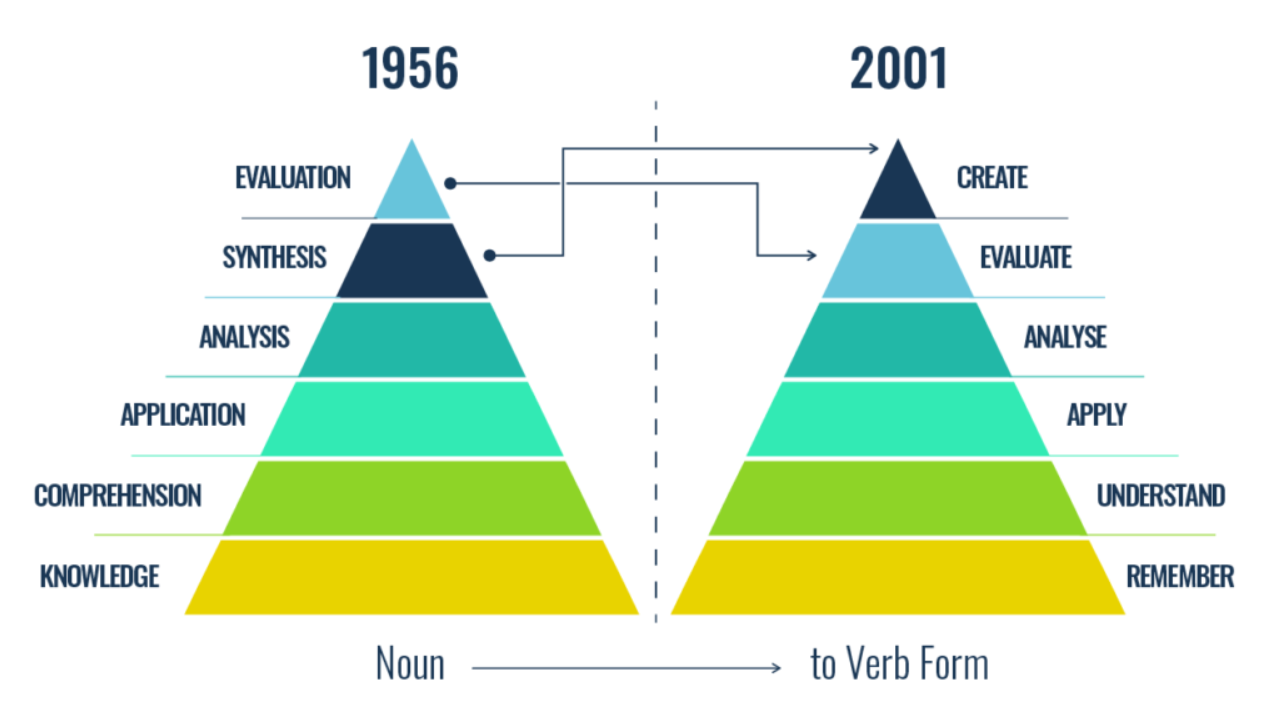
\includegraphics[scale=0.575]{blooms}
\caption{Comparison between Bloom's original Taxonomy and the revised version \cite{bloom-picture}} \label{fig:blooms}
\end{figure}

The original classification can be seen on the left hand side of Figure \ref{fig:blooms}. Each layer dictates that certain tasks will be able to be completed once the layer has been mastered. These are the skills obtained.

\textbf{Knowledge} is the most basic and fundamental skill one must obtain. This objective is the backbone for all others, one needs to be able to remember requisite facts in order to obtain more complex understanding. Some skills gained from this level could be: definition, description, identification, and recollection.

\textbf{Comprehension} is the next level, it suggests a student needs more than to just blindly recall facts, they need to understand a certain logic behind them. They need to be able to describe the meaning behind statements and explain this to someone. Skills gained in this tier include: description, explanation, summarisation, and discussion.

\textbf{Application} is the execution of a certain procedure. This is the first part of the Taxonomy where students may not know the answer directly, instead they must use their prior knowledge to solve certain problems. Necessary skills to prove application has been obtained might include: execution, calculation, implementation and manipulation.

\textbf{Analysis} argues students should be able to break information into parts and draw conclusions from connections between these parts. This might be different topics in a module, or points in an argument.  This is more advanced than application, since that skill was also on the recollection of steps of a procedure. Here students must generate their own conclusions, generating novel information. Skills gained here include: categorisation, comparison, deduction and criticism.

\textbf{Synthesis} is the next learning objective. This describes the process of creating new information. It involves organising knowledge in new ways to create a new piece of information, or a product. This skill may be required, in part, in the previous tiers, but truly creating something new is a skill all in its own. Skills that fall under this category might be: design, development, planning and invention.

\textbf{Evaluation} is the final learning objective in the 1956 version of Bloom's Taxonomy. In Bloom's handbook, evaluation is defined as ``the making of judgments about the value of ideas, works, solutions, methods, material, etc.'' More plainly, it is the skill of critiquing things, something that can only be done effectively when your knowledge is at the most sophisticated level. This is why Bloom and his team put it at the peak of the taxonomy. Some of the skills one must be able to demonstrate in order to prove evaluation is satisfied, and hence a subject has been mastered are: justification, criticism, judgement and assessment.

This describes the full taxonomy when it was created. It can be clearly seen that each one flows into the next, but there is also some overlap between these levels. For instance, the skill of description could fall under knowledge or comprehension, since a student could remember a certain description which shows knowledge, but could also suggest understanding if it wasn't blindly quoted. This is why the taxonomy is not a strict rule-set for learning. Instead, it is a measurement of progress and any curriculum using it should be implemented with care, instead of blindly following the pyramid.

\subsection{Revised Bloom's Taxonomy}

Much later, in 2001, Lorin Anderson led a new team of educators to update the taxonomy, called the Revised Bloom's Taxonomy (RBT) \cite{revised-blooms-taxonomy}. The structure, and differences between the original taxonomy can be seen in Figure 1.1. They opted to simplify some of the language, breaking down one potential barrier to the taxonomy's use. They also opted to replace the abstract verbs with present tense versions of the same words. More importantly, it was decided that creation was a more complex skill than evaluation.

In addition to the rearrangement of learning objectives, a new dimension was added to make a so called ``Taxonomy Table''. This new dimension is called the knowledge dimension, while the original is called the cognitive process dimension. \newline

\colorlet{Gray1}{black!90}
\colorlet{Gray2}{Gray1!80}
\colorlet{Gray3}{Gray2!80}
\colorlet{Gray4}{Gray3!80}
\colorlet{Gray5}{Gray4!70}
\colorlet{Gray6}{Gray5!60}
\colorlet{Gray7}{Gray6!50}
\colorlet{Gray8}{Gray7!50}
\colorlet{Gray9}{Gray8!0}

\begin{figure}[h]
\begin{center}
\begin{tabular}{|c|c|c|c|c|c|c|}
\hline
\multirow{2}{*}{\textbf{Knowledge}}& \multicolumn{6}{c|}{\textbf{Cognitive Process}}  \\ \cline{2-7}
& Remember & Understand & Apply & Analyse & Evaluate &  Create \\ \hline 
Factual & \cellcolor{Gray9} & \cellcolor{Gray8} & \cellcolor{Gray7} & \cellcolor{Gray6} & \cellcolor{Gray5} & \cellcolor{Gray4} \\ \hhline{*7-}
Conceptual & \cellcolor{Gray8} & \cellcolor{Gray7} & \cellcolor{Gray6} & \cellcolor{Gray5} & \cellcolor{Gray4} & \cellcolor{Gray3}  \\ \hhline{*7-}
Procedural & \cellcolor{Gray7} & \cellcolor{Gray6} & \cellcolor{Gray5} & \cellcolor{Gray4} & \cellcolor{Gray3} & \cellcolor{Gray2} \\ \hhline{*7-}
Meta-Cognitive & \cellcolor{Gray6} &\cellcolor{Gray5} &\cellcolor{Gray4} &\cellcolor{Gray3} & \cellcolor{Gray2} & \cellcolor{Gray1} \\ \hhline{*7-}
\end{tabular}\caption{Taxonomy Table for Bloom's Revised Taxonomy}\label{fig:brt}
\end{center}
\end{figure}

Figure \ref{fig:brt} shows the taxonomy table, with the new knowledge dimension. The shading refers to the complexity of each skill, darker being more complex. The knowledge dimension refers to the \textit{type} of knowledge used at that level, while the cognitive process dimension refers to \textit{how} that knowledge should be used. For instance, for one to have mastered the apply column, they must be able to apply factual, conceptual, procedural, and meta-congitive knowledge. \textbf{Factual} knowledge refers to the most basic information a student must be familiar with. It includes simple definitions, terms and symbols. \textbf{Conceptual} knowledge is the kind of knowledge one gains by understanding relationships between definitions. A lot of mathematics lies here, laws and theorems are examples of this kind of knowledge, but scientific theories, and more advanced, composite definitions also belong here. \textbf{Procedural} knowledge refers to processes. This is the knowledge needed to perform algorithms and tasks. It also includes techniques, methods and the understanding of when such processes need to be performed. Finally, the most advanced type of knowledge is \textbf{meta-cognitive} knowledge. This refers to knowledge about one's own learning. It includes the understanding of a student's own strengths and weaknesses, how they learn best, and even how to teach others effectively. It also contains knowledge about knowledge itself, for instance the structure of material in a course or material that will appear on certain tests.

Another problem Anderson and his team set out to solve the potential ambiguity within each of the definitions. They subdivided each item in the knowledge dimension into two or three ``sub-types'' and also divided each of the cognitive processes into categories, of which there were anywhere from two to seven. For instance, within analyse there are the categories of ``differentiating'', ``organising'', and ``attributing''. This would certainly help any potential educator planning to use the taxonomy table. Needless to say, it was a rigorous overhaul and one of many overhauls Bloom's taxonomy has received since its original publication.

\section{Learning Resource Requirements}

With the aid of Bloom's taxonomy, and a few other sources it should be possible to outline the requirements of a good learning resource. These will be the guidelines will be attempted to be met, and will be evaluated against in the Results Section. The definition of learning resource used here is specifically an article, textbook, or tutorial used for self-teaching. Not included here are things like videos, or spoken word, which have their own additional criteria. See Section \ref{section:ideasForFutureWork} for more information on other possibilities that could be explored.

These are 9 aspects that contribute to the effectiveness of a learning resource under this definition:

\begin{itemize}
    \item \textbf{Good readability} 
        \begin{itemize}
            \item Readability is a measure of how easy a text is to read. A highly readable text will have shorter sentences and simpler vocabulary. If a text is readable, it means that information can be conveyed more directly allowing otherwise difficult ideas to be explained simply. One should note however, that academic subjects do have a high level of complexity and often cannot be explained in a particularly readable way. Therefore, the goal is to maximise readability, while still conveying all the intended information.
        \end{itemize}
    \item \textbf{Effective use of visual learning methods}
        \begin{itemize}
            \item One way to aid a student in understanding difficult ideas is through visualisation. Color, graphs, flow charts, diagrams, and more, all fall under the umbrella of visual learning approaches. They provide a new way of thinking about certain ideas, allowing readers to more easily pick up the information \cite{times-higher-education}.
        \end{itemize}
    \item \textbf{Professional aesthetics}
        \begin{itemize}
            \item While aesthetics are not all that important and the information and explanations are the key content, they are still relevant when listing important attributes of a good learning resource. This is because information on the page should not be cluttered or distracting, the focus should be on content such as text, diagrams, animations and code snippets.
        \end{itemize}
    \item \textbf{Good pacing}
        \begin{itemize}
            \item A good learning resource shouldn't move too quickly through content, otherwise students may feel unprepared for new concepts. A fair amount of time should be spent on examples and explanations in order for students to fully consolidate the information. Care should also be taken however, to not slow down the pace too much. Spending too much time on an individual idea might cause the student to lose interest or start skipping through sections.
        \end{itemize}
    \item \textbf{Proof of usefulness}
        \begin{itemize}
            \item The ultimate aim of a learning resource is for a student to take the knowledge they gain from it and gain a practical skill. Even some of the most pure mathematical fields have practical applications. Students want to know how the information presented actually links to real problems. \cite{times-higher-education}
        \end{itemize}
    \item \textbf{Well-tuned difficulty}
        \begin{itemize}
            \item This section certainly links to pacing, the content should not feel difficult because the student is unprepared. However, another point to note is that any exercises provided should not be too difficult, while providing a challenge at the same time. There should be a range of questions that test the student in the subject matter, having a level of difficulty that ranges as far as the student is willing to go.
        \end{itemize}
    \item \textbf{Sensible structure}
        \begin{itemize}
            \item The flow of the learning resource should make sense. Not only from paragraph to paragraph but from section to section. One should motivate the other, keeping the reader engaged and causing them to continue reading.
        \end{itemize}
    \item \textbf{Clear objectives defined}
        \begin{itemize}
            \item At the start of the resource, clear learning objectives should be set out. This would motivate the student to continue reading, since they will not only know what they will learn, but also how they will be able to apply it. Then, at the end, students will be able to reflect on these objectives and decide for themselves whether or not they have achieved them.
        \end{itemize}
\end{itemize}

%MEANS I NEED TO DEFINE EXACTLY WHAT MAKES A GOOD LEARNING RESOURCE, WHICH SHOULD HELP OUTLINE MY METHODS.

\section{Analysis of Existing FEM Learning Resources}

With a more precisely defined criteria of what makes a good learning resource, it is now possible to analyse some of the most popular learning resources in finite element analysis.

\subsection{Bengzon and Larson's Finite Element Textbook}

We start with a textbook written by Mats. G. Larson and Fredrik Bengzon called The Finite Element Method: Theory, Implementation, and Applications \cite{bengzon-larson-fem}. This textbook is meant to introduce students to the finite element method by explaining the necessary mathematics, while also showing how to implement it in MATLAB. 

The textbook seems to meet most, if not all criteria listed above. It has decent readability and aesthetics. Visuals have been used well throughout, the diagrams of finite element basis functions are particularly useful. The difficulty is kept to a minimum. This is due to excellent pacing that begins by introducing the problem in a 1D example, then moves up to 2D, giving readers ample time to digest the methods presented. These first five chapters give enough information for a student to be able to implement most simple PDEs. Information after this gets more advanced, and several chapters are devoted to specific engineering problems. This also gives the reader some real world context to FEM, making the reading significantly more engaging.

At the end of each chapter a selection of exercises are presented. These are very well written, allowing the reader to consolidate information gained in the previous chapter. Bloom's Taxonomy seems to be mostly satisfied, there are questions relating to simple recollection and use of definitions (recall), and to applying methods learned to specific problems (comprehension and application). In questions that require the reader to construct a proof, analysis is met because, one must bring together several concepts and ideas to construct an argument. Synthesis could also be considered to be part of proof-writing, although the definition might be being stretched here. Evaluation however, is not so well explored. This could be one criticism against the book. Bengzon and Larson could have asked students which approach might be better for certain problems for instance, which would force the reader to weigh up the advantages and disadvantages of certain methods.

\subsection{J. S. Dokken's FEniCSx Tutorial}

The next FEM learning resource is a tutorial specifically written as a guide for FEniCSx, the previously mentioned FEM computing platform. It is written and maintained by Jørgen S. Dokken, a researcher in the field and member of the FEniCSx Steering Council. The tutorial was adapted from Langtangen and Logg's book \textit{Solving PDEs in Python: The FEniCS Tutorial I} \cite{langtangen-logg}, which was written for the previous version of FEniCSx.

Rather than as a guide to the finite element method, this tutorial serves more as a guide on how to use FEniCSx. Having said that, mathematical explanations are provided, they are just simply not as detailed as Bengzon-Larson for instance. The tutorial is written using in a Notebook format, which is spoken about in Section \ref{section:jupyter}, but means that code snippets feature heavily. Dokken uses a service called Binder to host the notebooks remotely, which allows users to run the code in their own browsers without downloading any dependencies. This removes a large barrier to the use of FEniCSx, and lets users tinker and get familiar with the library without having to download the libraries on their local machine. If one does not wish to use Binder, they are free to view the static version as well.

The notebook is very readable, jargon is kept to a minimum, although there is still quite a lot due to the subject matter. Many terms are hyperlinked to external sites where readers can find more detailed information. Visuals are used vary sparingly, which is one downside of the tutorial. It could certainly be improved with a few diagrams or illustrations. The pacing is excellent, and each chapter uses information from the previous to expand the reader's knowledge in an engaging way. Sometimes the pace can be slightly too fast, and important concepts don't have enough time spent on them, but in these cases external resources are often linked to, and Dokken recommends that readers unfamiliar with FEM read a textbook on the subject.

The usefulness is motivated fairly well, there is a section titled ``Gallery of Finite Element Solvers'' which provides plenty of examples. Most of the problems presented however seem to be idealised, but still provide good insight into the potential applications of FEniCSx. The sections flow well between each other, and difficulty is well managed. Learning objectives also feature at the start of every chapter, which is great to see.

% ANY BRILLIANT/CODACADEMY/UDEMY TYPE STUFF THAT COULD BE RELEVANT (VECTOR CALCULUS OR PYTHON).